\section{Structure}
In this section we will be describing the overall structure of the program, through class diagrams.

\subsection{Individual class description}
In this subsection the different classes will be described with a short text.

\begin{figure}[H]
	\centering
	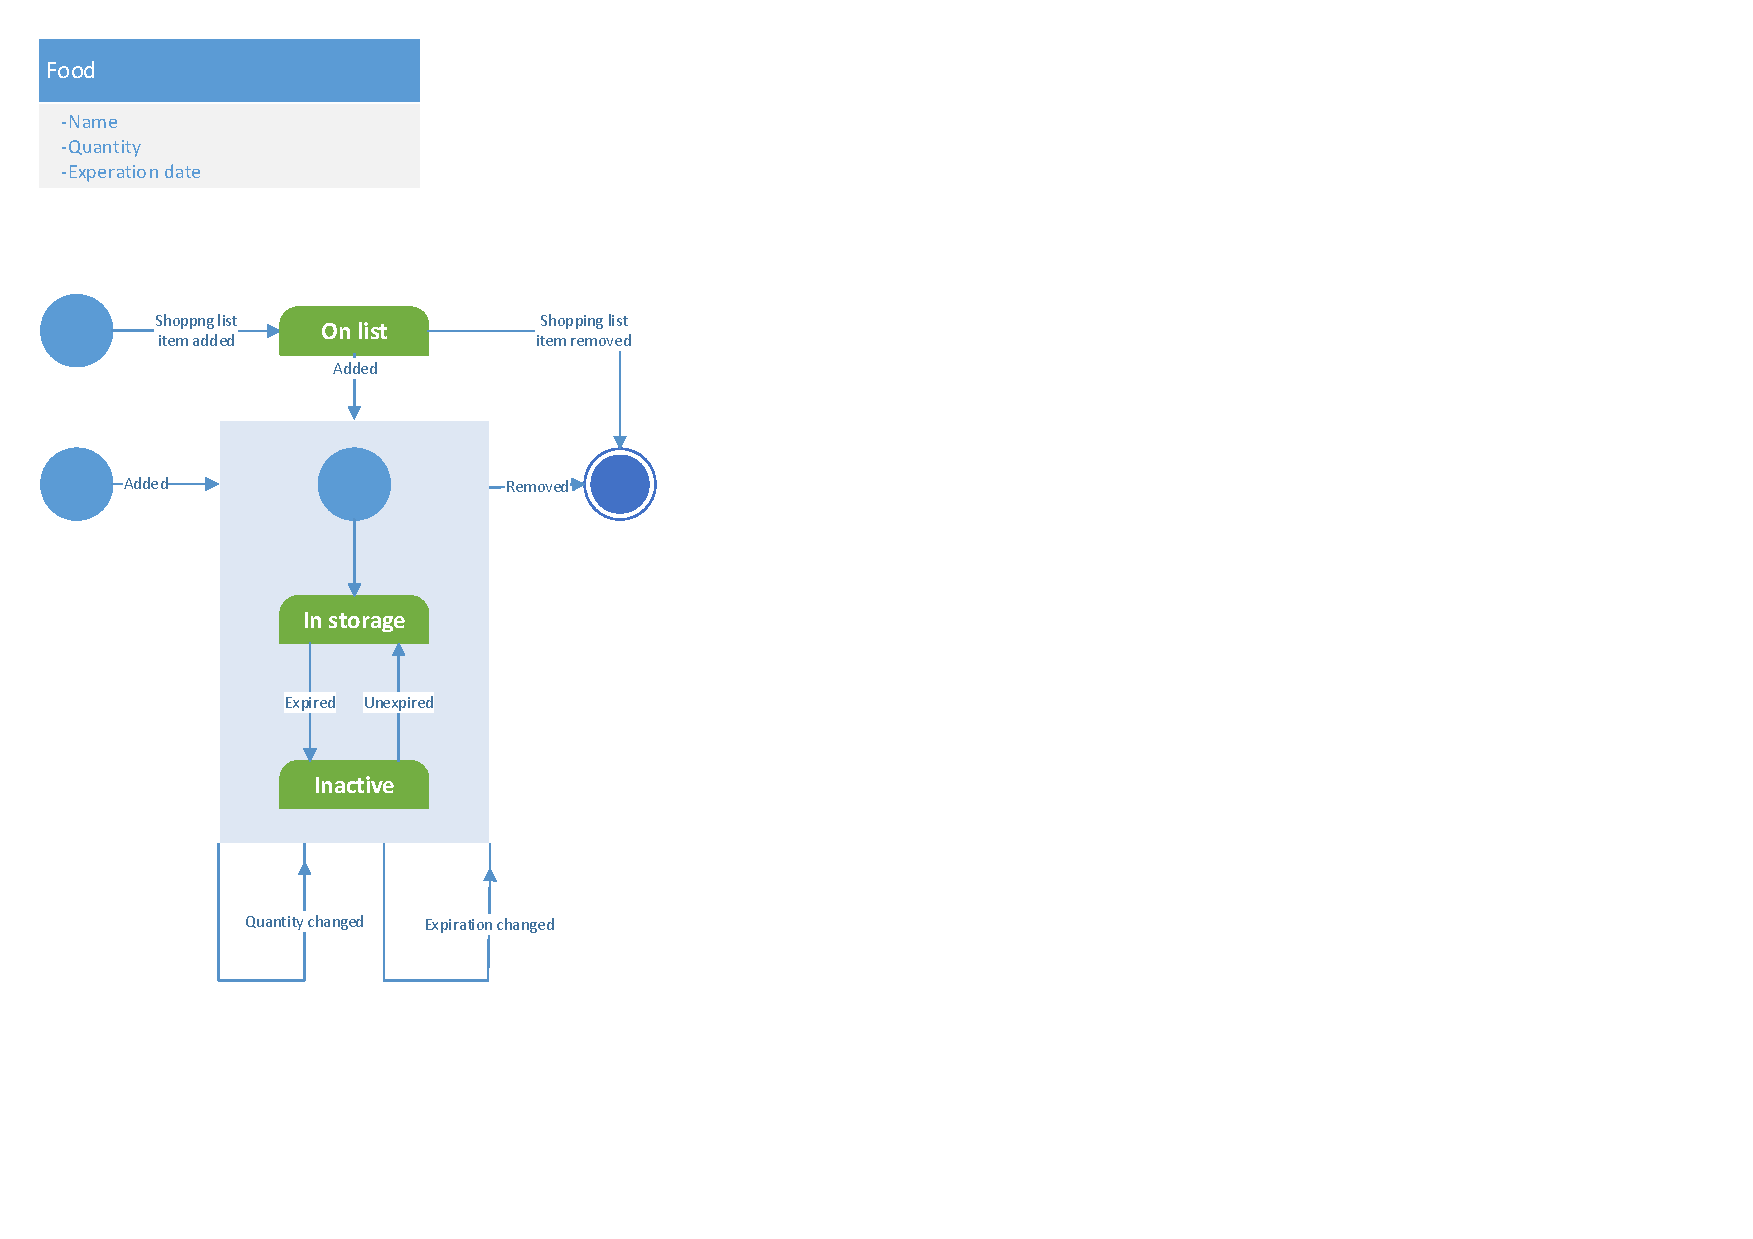
\includegraphics[width=1.0\textwidth]{Development/ProblemDomain/FoodClass.pdf}
	\label{FoodClass}
\end{figure}
The \textbf{Food} class contains information about the quantity and expiration date of an food item. The food items can be found on the lists inventory or shopping list.

\begin{figure}[H]
	\centering
	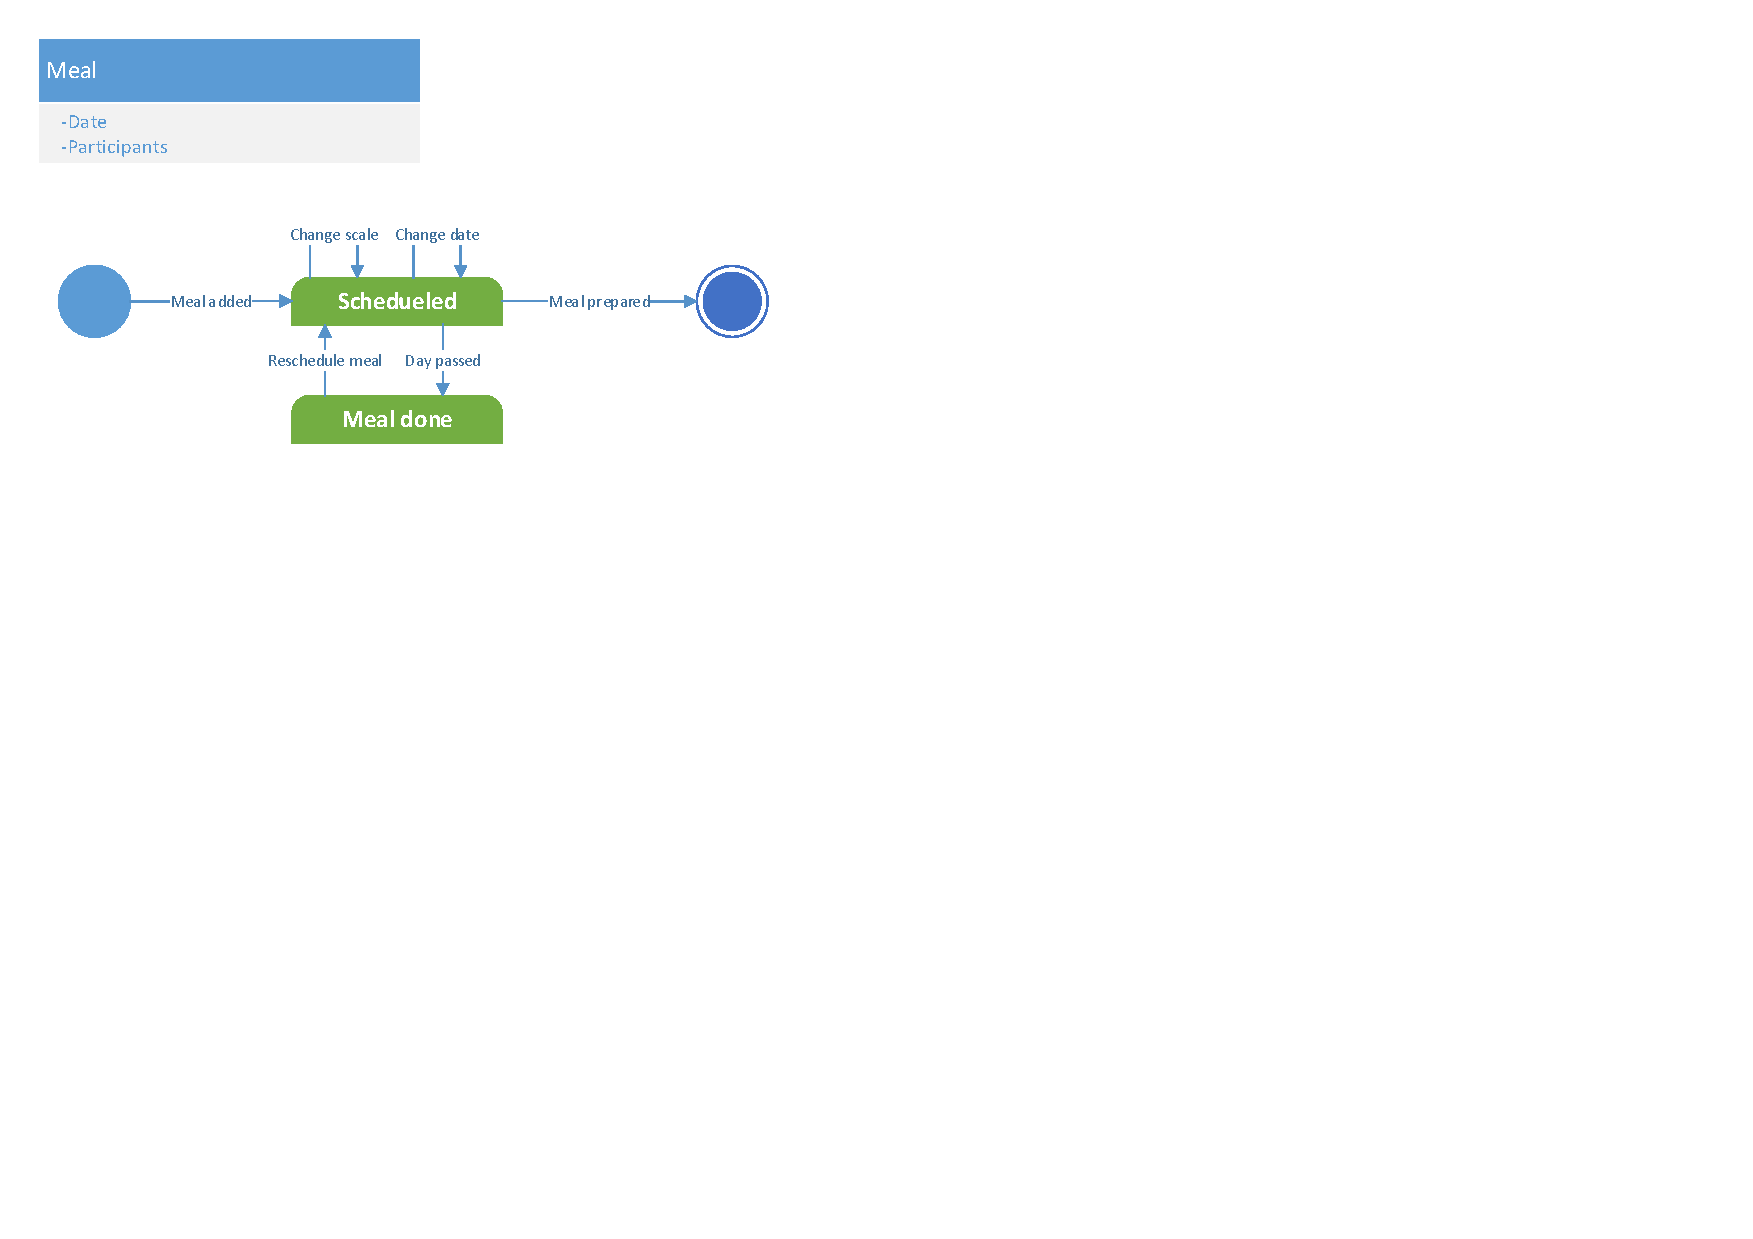
\includegraphics[width=1.0\textwidth]{Development/ProblemDomain/MealClass.pdf}
	\label{MealClass}
\end{figure}
The \textbf{Meal} class contains information about a meal and when to make it. It consists of recipes.

\begin{figure}[H]
	\centering
	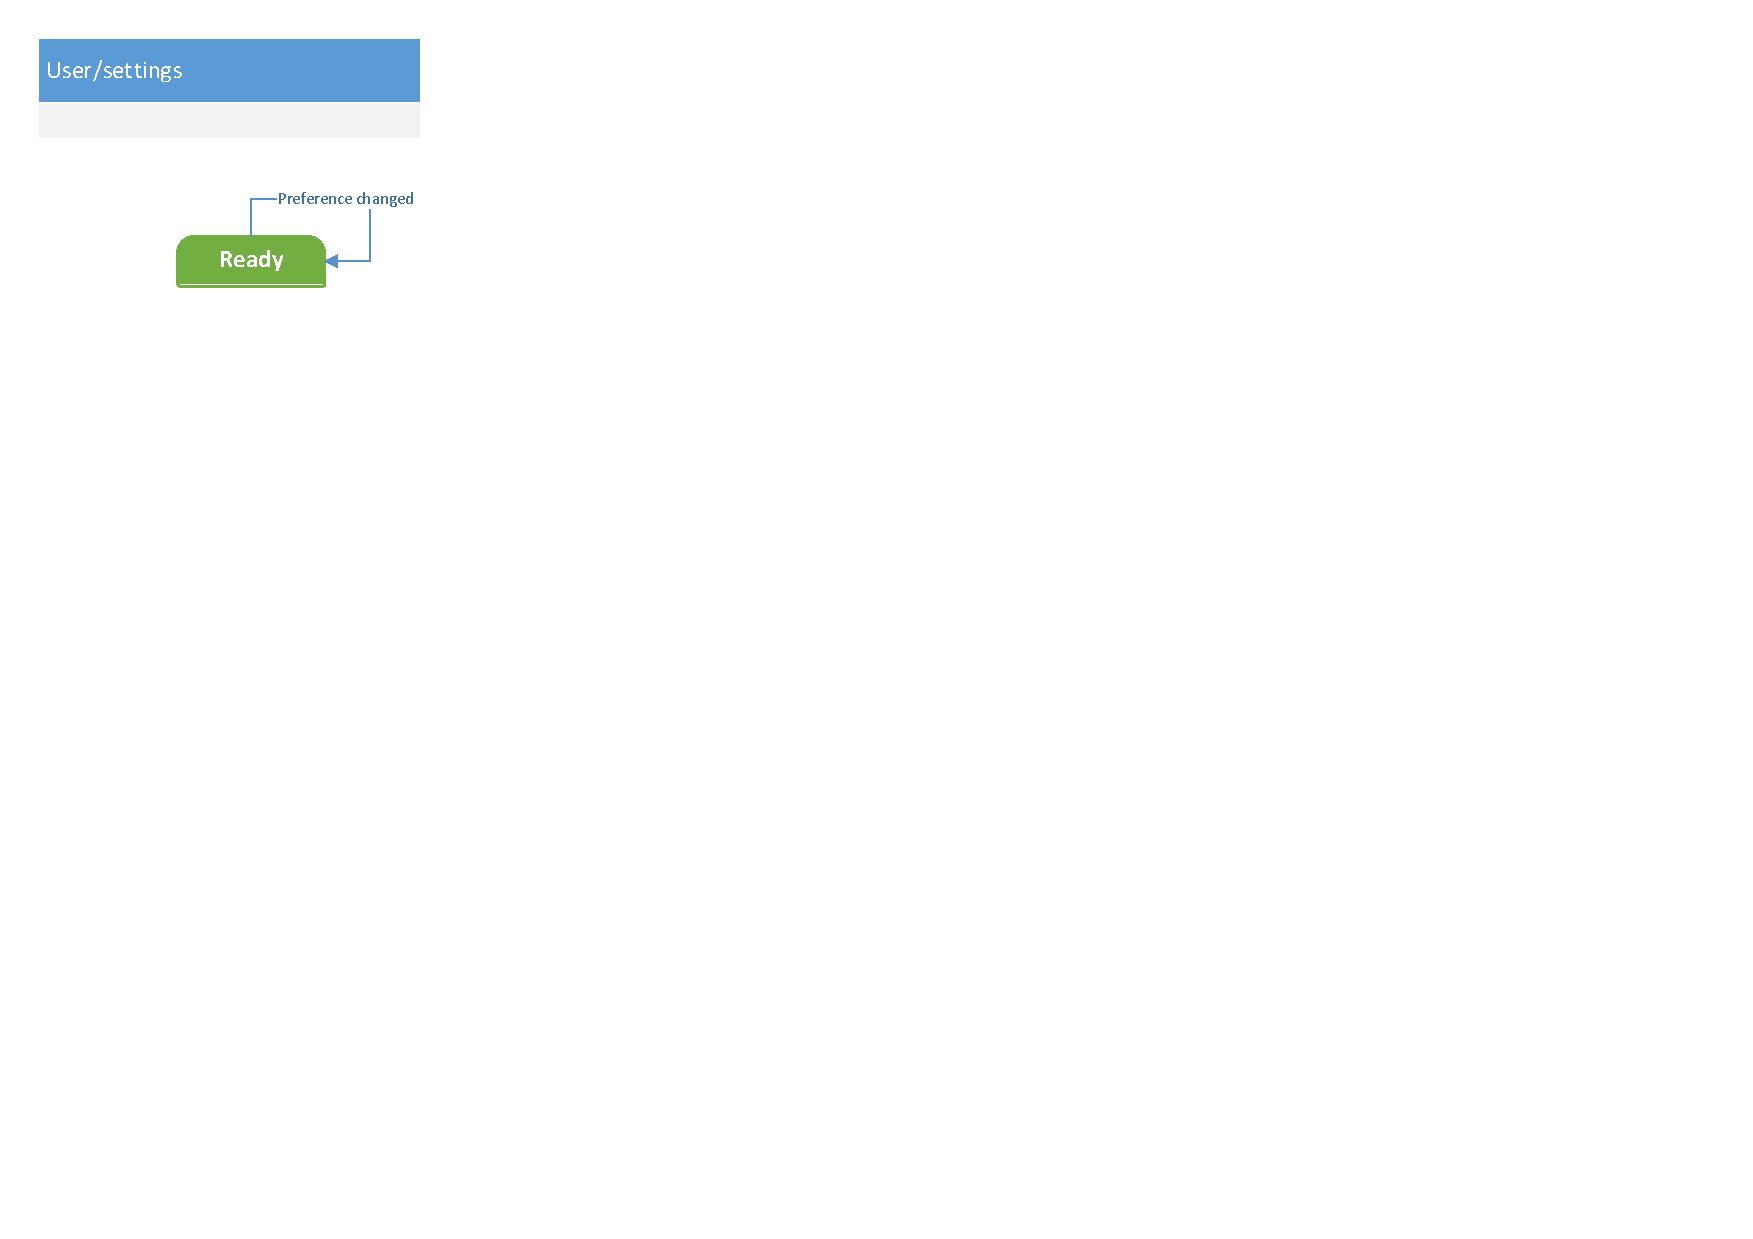
\includegraphics[width=1.0\textwidth]{Development/ProblemDomain/UserSettingsClass.pdf}
	\label{UserSettingsClass}
\end{figure}
The \textbf{User settings} class contains preferences from the user which the system should take into consideration.

\begin{figure}[H]
	\centering
	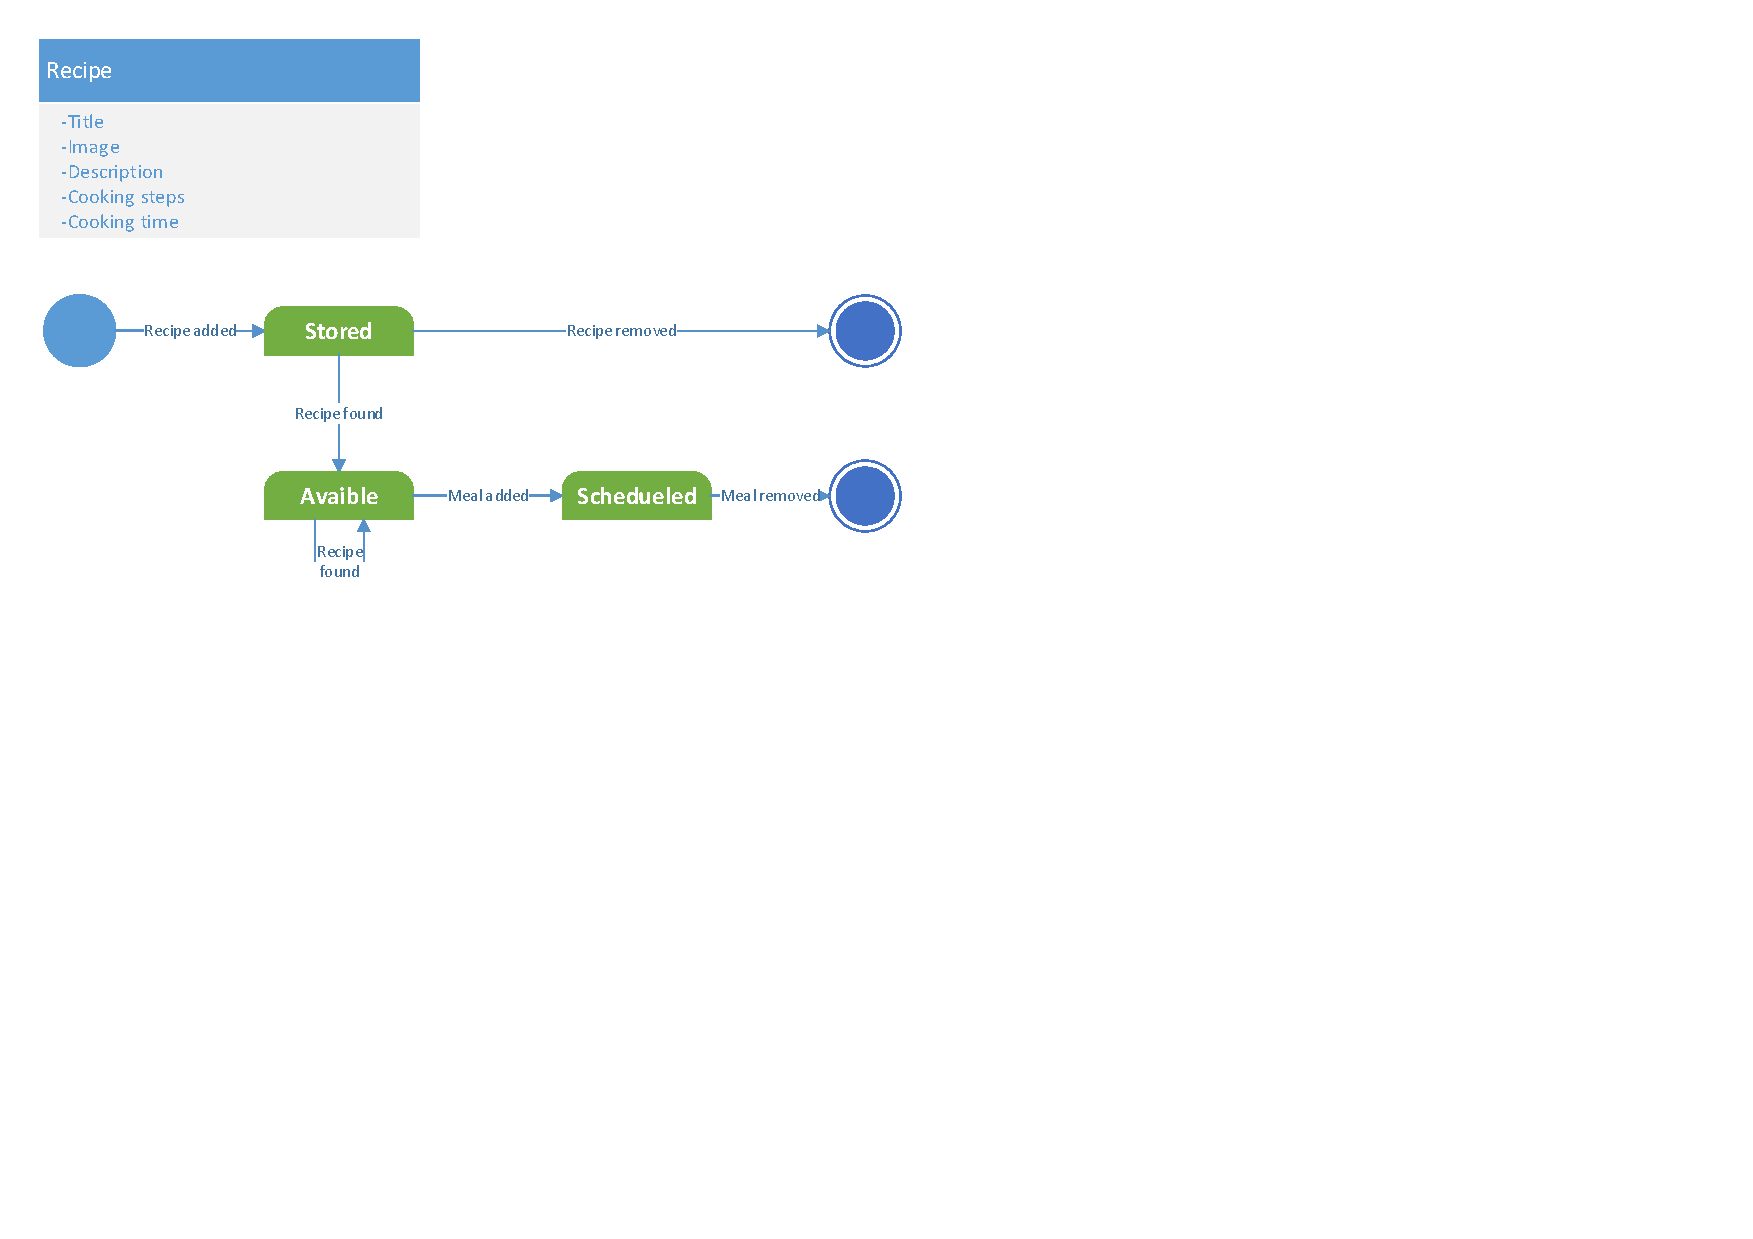
\includegraphics[width=1.0\textwidth]{Development/ProblemDomain/RecipeClass.pdf}
	\label{RecipeClass}
	\end{figure}
\textbf{Recipes} consists of \textbf{Food}. It also contains information on how to prepare the meal from the recipe.

\subsection{Class diagram description}
The class diagram is structured with \textbf{Food} as the central class. 
\textit{Shopping List}, \textit{Inventory} and \textit{Foodplan} are lists, containing \textit{Food} or \textit{Meal}.

Food objects can be part of a \textbf{Shopping List}, a user \textbf{Inventory}, or be part of a \textbf{Recipe}, seen as aggregation on \cref{fig:classDiagram}. A \textbf{Recipe} contains 1 to many Food objects, and is part of a \textbf{Meal} that in turn is part of a \textbf{Foodplan}. A \textit{Meal} contains exactly 1 recipe, while the \textit{Foodplan} can have any number of planned \textit{Meals}.

\fxnote{fix references..}
\begin{figure}[H]
	\centering
	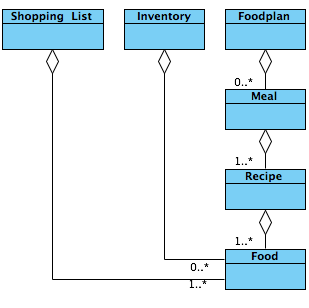
\includegraphics[width=0.50\textwidth]{Grafik/FoodPlanner/FoodPlannerClassDiagram.png}
	\caption{Relation between classes.}
	\label{fig:classDiagram}
\end{figure}